\documentclass{standalone}
\usepackage{tikz}

\begin{document}

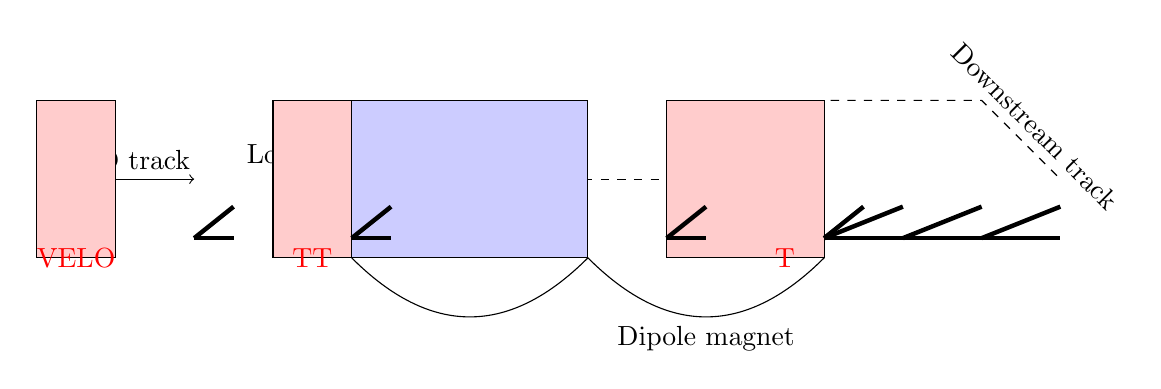
\begin{tikzpicture}[scale=1]
    % Draw the VELO track
    \draw[->] (-4,0) -- (-2,0) node[pos=0.5,above,sloped] {VELO track};
    
    % Draw the TT track
    \draw[->] (-1,0) -- (0,0) node[pos=0.5,above,sloped] {Long track};
    
    % Draw the downstream track
    \draw[dashed] (0,0) -- (4,0);
    \draw[dashed] (4,0) -- (6,1) -- (8,1) -- (9,0) node[pos=0.5,above,sloped] {Downstream track};
    
    % Draw the T track
    \draw[->] (4,0) -- (6,0) node[pos=0.5,above,sloped] {T};
    
    % Draw the VELO detector
    \draw[fill=red!20] (-4,-1) rectangle (-3,1);
    \node at (-3.5,-1) {\textcolor{red}{VELO}};
    
    % Draw the TT detector
    \draw[fill=red!20] (-1,-1) rectangle (0,1);
    \node at (-0.5,-1) {\textcolor{red}{TT}};
    
    % Draw the Dipole magnet
    \draw[fill=blue!20] (0,-1) rectangle (3,1);
    \draw (0,-1) .. controls (1,-2) and (2,-2) .. (3,-1) .. controls (4,-2) and (5,-2) .. (6,-1) node[pos=0.5,below,sloped] {Dipole magnet};
    
    % Draw the T detector
    \draw[fill=red!20] (4,-1) rectangle (6,1);
    \node at (5.5,-1) {\textcolor{red}{T}};
    
    % Draw the tracks with bars
    \foreach \x in {-2,0,6} {
        \draw[black,ultra thick] (\x,-0.75) -- (\x+0.5,-0.75);
        \draw[black,ultra thick] (\x,-0.75) -- (\x+0.5,-0.35);
    }
    \draw[black,ultra thick] (4,-0.75) -- (4.5,-0.75);
    \draw[black,ultra thick] (4,-0.75) -- (4.5,-0.35);
    
    \draw[black,ultra thick] (6,-0.75) -- (7,-0.75);
    \draw[black,ultra thick] (6,-0.75) -- (7,-0.35);
    \draw[black,ultra thick] (7,-0.75) -- (8,-0.75);
    \draw[black,ultra thick] (7,-0.75) -- (8,-0.35);
    \draw[black,ultra thick] (8,-0.75) -- (9,-0.75);
    \draw[black,ultra thick] (8,-0.75) -- (9,-0.35);
    
    \end{tikzpicture}

\end{document}